\section{Data preprocessing}
\label{section:Method:Preprocessing}
This section briefly describes all the data processing done.

\subsection{Train, validation, test splitting}
% The training and validation datasets were seperated in a manner similar
% to that described by \cite{Bandara2019} and \cite[]{Hewamalage2021}.

The inspiration of the training, validation and test splitting is taken from
\cite{Bandara2019}, \cite{Hewamalage2021}.
Both reserve the last $m$ sized part of the training set as a validation set,
where $m$ is the forecasting window size.
% This means L - 2*(n+ m)
%\cite{Hewamalage2021} reserves the last $m$ sized part for validation,
%where $m$ is the forecasting window size.
However, \cite{Hewamalage2021} note that this is problematic.
This is because the last part of the training set is removed
and therefore not considered when training the model, as it is used only for validation during model selection and tuning.

The further away the test predictions are from the training set the worse,
because the underlying patterns may change during this last part of the sequence.
Therefore \cite{Hewamalage2021} suggests an alteration to the use of the validation split.
The validation set is split from the training set only when tuning the model,
and is thereafter added to the training data when the model is used and tested.
Thus, the models will be trained on all available data, excluding only the selected test set.

We did however make some modifications to the approach presented by \cite{Hewamalage2021}.
Initially, the complete dataset is available.
A test set, consisting of the last $m$ points of the sequence, is then manually split from the complete dataset.
After this, the training set is used to define both the used training set and the validation set.
For the SARIMA method, a validation split is not needed.
However, the use of an LSTM, specifically a stateful LSTM, causes restrictions to the creation of the validation set.
Due to the use of stateful LSTM modules, the validation set has to be the same batch size as the training set.
This, in turn, means that using a validation set equal to the forecasting window $m$ would limit the available batch size for the model
used on the training set.
\cite{Bandara2019} would always train their models on multiple time series,
which meant that their validation set would be $validation\_size = m * number\_of\_series$.
In contrast we would also train models on a single time series at a time.
In this case the validation set size would be equal to one forecasting window.
During development and testing it was found that a validation set size of only one forecasting window is exceedingly small.
Tuning on validation error would be severely limited and would produce models with less optimal hyper parameters.

As a result of these findings we selected a batch size for the training set beforehand, then
used the chosen batch size as a validation set size.

This, however, means that we are not able to conduct a hyperparameter search for an optimal batch size
because that would change the validation set as well.
When we tried this, the model would almost always prefer the smallest possible batch size because that meant
it would get a small validation set, which also reduced the number of possible errors it could make.

When tuning the models, the validation set is actively used as a measurement of the predictive ability of the model.
However, when conducting final experiments with well-defined models and parameters,
the validation set is once again added to the training set so that the model has more data to train on.
This is the same approach as used in \cite{Hewamalage2021}.


%part L - (IW + OW) as test set,
%and the next part for validation L - 2(IW + OW) during tuning.
%But for testing and prediction they will train on the validation set as well
%because the last part of the sequence is not considered for training the model.
%The further away the test predictions are frin the training set, the worse
%because the underlying patterns may change during this last part of the sequence.


\begin{figure}[h!]
  \centering
  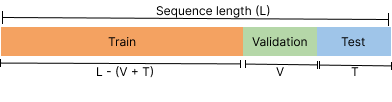
\includegraphics[width=0.7\textwidth]{./figs/illustrations/illustration_train_val_test_split.png}
  \hfill
  \caption{Illustration of trainig, validation, and test split. V = batch size, T = m = forecast window}
  \label{fig:train-val-test-split}
\end{figure}

\Cref{fig:train-val-test-split} shows an illustration of how one dataset is split up during
hyperparameter tuning.
The whole time series has a size of length $L$. The test set $T$ is taken from the end of the series,
and has the size of the forecast window $L = m$. The validation set $V$ has the size of
one batch size $V=batch\_size$. So during tuning the size of the training data is
$T = L - (V + T)$. During testing the validation set $V$ is re-added to the training set,
making the training set $T = L - T$.

\begin{figure}[h!]
  \centering
  
\includegraphics[width=0.7\textwidth]{./figs/illustrations/illustration_global_time_series.png}
  \hfill
  \caption{Illustration of how multiple time series are concatonated for the global method}
  \label{fig:global-time-series}
\end{figure}



\subsection{Feature Engeneering}
Both the feature \textit{"hits"} and \textit{"clicks"} can be argued to measure
user interest. A product's hits score measures how many times someone has clicked
on that product information page at prisuigen.no. A product's click score to measure
how many times prisguiden.no has redirected a user to an external retailer for the given product.
We ended up combining these two variables into one feature which we called \textbf{"interest"}
with the equation defined in \Cref{eq:interest}.
\begin{equation}
  interest = hits + clicks
  \label{eq:interest}
\end{equation}




\subsection{Value Scaling}
\label{section:Data:Preprocessing:value-scaling}
Deep learning models require appropriate scaling to converge properly.
For the neural networks we scaled the data using standardization.

\begin{equation}
  z = \frac{x - \mu}{\sigma}
\end{equation}
Where $\mu$ is the mean and $\sigma$ the standard deviation.

\begin{equation}
  x\_std = \frac{x - x.min()}{x.max() - x.min()}
  x\_scaled = x\_std * (h - l) + l
\end{equation}
where $h$ is the max feature range and $l$ is the min.

For scaling data, two different approaches were explored.
Both normalization and standardization were explored.
As the data distribution is not known prior to the scaling, normalization ensures a known value range for scaling.
For the neural net models we scale using normalization for the ranges to be in the range [0.1, 1].
The unconventional choice of having 0.1 as our lower bound is because the matric SMAPE
is vulnerable to zero values, as described in \Cref{eq:sMape}.

However, during experimentation and testing, it was found that scaling with standardization
outperformed the predictions made with a normalization scaling.
Both methods were explored, but at last standardization was selected as the scaling method.



\iffalse
  Standardization was chosen over normalization because experiments showed better perfomance with
  standardization.

  For the neural net models we scale using normalization for the ranges to be in the range [0.1, 1].
  The unconventional choise of having 0.1 as our lower bound is becuase the matric SMAPE
  is vulnerable to zero values, as described in \Cref{eq:sMape}.

  Normization was chosen over standardization because we do not know the distrubtion
  of the data, and we did not want to assume it followed a Gaussion distribution.
  All model output and predictions are rescaled to it's original range before
  visualizing and plotting.
\fi

%%% This should not be needed. This should be defined in the ARIMA pipeline / method / experiment.
%%% This is only what different types of changes were done to the datasets at different points
%For the ARIMA models we did not scale the data because ARIMA models will not
%get the same benefits by scaling the input data.

%The way our data pipeline was constructued made it self documenting,
%which means it prints out all the processing steps and saves them as the
%experiment is conducted. This section will briefly cover how the data was processed
%before each type of experiments.
%The different model structures required some differences in processing steps.




\subsection{Univariate to Multivariate feature engeneering}
Since the E-commerce domain is heavily influenced by external factors, such as
holidays, Christmas, and yearly seasons we thought it would be beneficial
for the neural net models to be aware of which day of the week it is,
which month it is, and if it is closer to summer than winter.

We add the \textit{month} feature, a number between [0, 11] depending on which month.

We add the \textit{day} feature, a number between [0, 6] where 6 is saturday, 0 is sunday etc.
We can calculate the day of the week using the formula \Cref{eq:day_of_the_week}
from \Cref{section:BT:day-of-the-week-formula}.

We add the feature \textit{season} which is a number between [-1, 1] using \Cref{eq:season_feature}.

\begin{equation}
  season = \cos(\pi * (month \mod{12}) / 6)
  \label{eq:season_feature}
\end{equation}

\begin{figure}[h!]
  \centering
  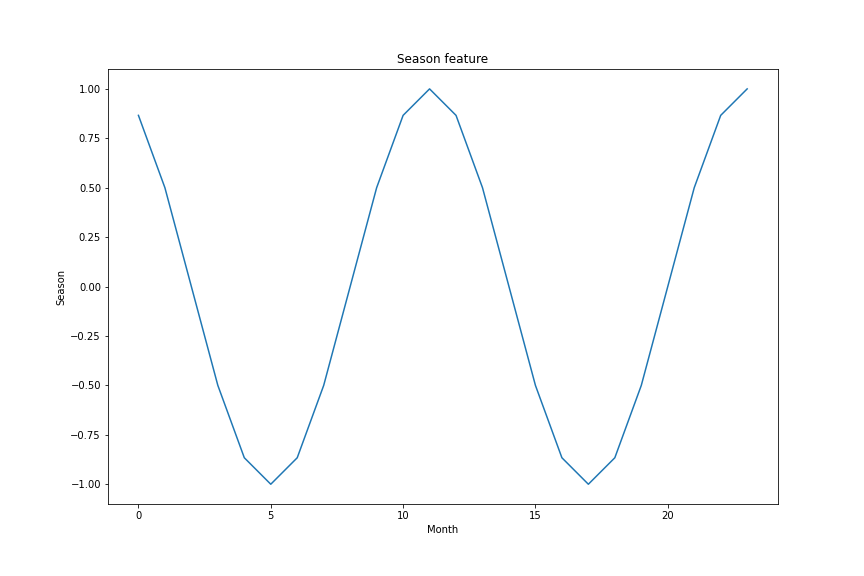
\includegraphics[width=\textwidth]{./figs/code_generated/season_feature.png}
  \hfill
  \caption{Season feature}
  \label{fig:season-feature}
\end{figure}

\Cref{fig:season-feature} shows the output of the season feature.
If the month is close to Christmas (december, januar) this feature will be close to 1.
If the month is closer to summer (may, june) this feature will be close to -1.

In the and all added features are scaled between [0.1, 1] as described above.


\subsection{Moving Window Approach}
\label{section:Data:Preprocessing:moving-window-approach}
When creating the datasets, we apply the same moving window approach as applied by \cite{Bandara2019} and \cite{Hewamalage2021}.
This strategy transforms a time series $X_i$ into pairs of $<input, output>$ patches.
In other words we transform the problem into a supervised learning problem [\Cref{fig:dataset:moving_window_scheme}].

Given a time series $X_i = \{x_1, ..., x_K\} \in \mathbb{R}^K$ of length $K$ a mowing
window algorithm will convert the time series $X_i$ into $K-n-m$ number of patches,
where each patch has the size of $m+n$, and $n$ is the size of the input window,
and $m$ is the size of the output window.

This thesis will primarily work with an output windows $m$ for size 7.
This is because it is safe to assume that the E-commerce domain consists of weekly patterns.
7 days is short enough that we should be able accurately to forecast something meaningful,
but long enough to have some commercial value.

\cite{Hewamalage2021} suggests setting the input window size $n$ to be slightly
bigger than the input window with $m * 1.25$. Or putting $m$ slightly bigger than
the seasonality period $m = 1.25 * seasonality\_period$.
We selected to make the input window a bit bigger than the output window and the weekly
period, by setting $m = 10$.
\begin{figure}[h!]
  \centering
  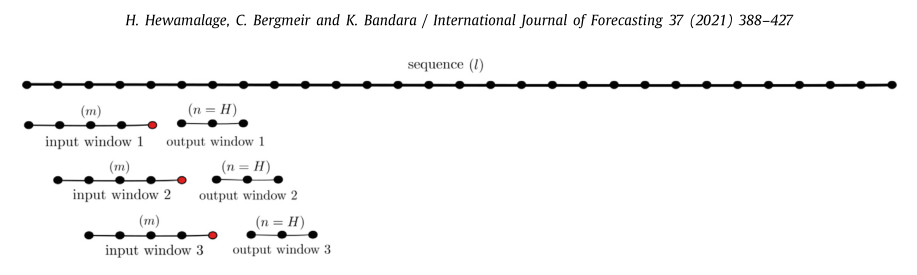
\includegraphics[width=\textwidth]{./figs/illustrations/moving_window_illustration.png}
  \hfill
  \caption{Moving window scheme \citep{Hewamalage2021}}
  \label{fig:dataset:moving_window_scheme}
\end{figure}



\subsection{Modeling Trend and Seasonality}
\label{section:Data:Preprocessing:trend-and-seasonality}

\todo[inline]{This reads a lot like a section from Related Work. Should it be moved?}

The literature is conflicting when it comes to NNs capability to
model trends and seasonality. \cite{Sharda1992} work inferred that NNs are
capable of modeling seasonality accurately.
However, more recent work suggests that deseasonalisation and
detrending can boost performance of neural networks [\cite{Zhang2005} \cite{Smyl2020}].
\cite{Ouyang2021} show that detrending and deseasonalisation using STL decomposition
will harm machine learning models, but improve statistical models.

\cite{Hewamalage2021} conclude that when all the series in a dataset follow
homogeneous seasonal patterns, with all of them covering the same duration in time
with sufficient lengths, RNNs are capable of capturing seasonality
without prior deseasonalisation.
If this is not the case then RNNs have a hard time modeling
seasonality on their own, and deseasonalisation step should be employed.

\cite{Montero-Manso2021} advocates for not removing seasonality on global models based on their empirical results.
They conclude that global NNs do not suffer from an inability to pick seasonal patterns,
as long as the models are sufficiently complex and have enough memory. They argue that removing
seasonal patterns from the data can erase some relevant information that might be exploited by global models.

\cite{Hewamalage2021} experiments on NNs ability to model seasonality show that NNs are capable of
modeling seasonality on their own, when all the series in the dataset have similar seasonal patterns.
When this is not the case deseasonalisation and detrending should be removed.

These conflicting results in the literature, combined with our varied set of time series
we conclude that we will avoid applying STL decomposition in our main experiments,
but might do some experiments to see how it can improve our metrics.
% TODO: Write about differencing and how it removes trend and seasons

\subsection{Scaling down outliers}
\label{section:Data:Preprocessing:scale-down-outliers}
Some of our time series consists of a few extreme outliers. An example of
how one of these outliers might occur is if a supplier makes an error and sends
a wrong price to Prisguiden. If this price is much lower than the original price then
it might spike a huge user interest for this item, until Prisguiden finds and corrects the error.
These outliers do not give any meaningful information, so steps were taken to reduce these extreme values.

We use the standard deviation as a base to scale down the outliers with the formula below.

$y(t_n)=
  \begin{cases}
    x * 0.3 & \text{if } x\geq standard\_devation * 5 \\
    x,      & \text{otherwise}
  \end{cases}$

An example of how this affects a time series is shown in \Cref{fig:illustration:scaled-down-outliers}.
\begin{figure}[h!]
  \centering
  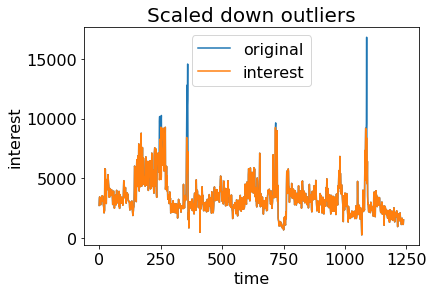
\includegraphics[width=0.5\textwidth]{./figs/code_generated/data_exploration/scaled_down_outliers.png}
  \hfill
  \caption{Illustration of how the scaling effects a time seires. The blue is the original series. The orange is the processed series.}
  \label{fig:illustration:scaled-down-outliers}
\end{figure}

\subsection{Data Processing Summary}
So far, we have described each processing step and how it is conducted, but not the overall
order.

The main preprocessing steps was carried out as follows:
\begin{enumerate}
  \item Combine \textit{hits} and \textit{clicks} to feature \textit{interest}.
  \item Split up into test and training data.
  \item If a multivariate model $->$ Generate date features.
  \item Scale down outliers %[\Cref{section:Data:Preprocessing:scale-down-outliers}].
  \item Normalize the data %[\Cref{section:Data:Preprocessing:value-scaling}].
  \item Generate sliding window patches %[\Cref{section:Data:Preprocessing:moving-window-approach}].
  \item Split the training set into training and validation set.
\end{enumerate}

If the model is a global model. Then the same steps described above are executed once
for each time series, and then the training sets, validation sets, and test sets are concatenated.

The post-processing on the predicted forecasts is just a matter of reversing the local
normalization to the forecast.
